\documentclass[12pt,a4paper]{article}

\usepackage{tikz}
\usetikzlibrary{shapes.geometric, arrows.meta, fit, backgrounds, calc, positioning, shadows}

\begin{document}

\begin{figure}[htbp]
\centering
\scalebox{0.9}{
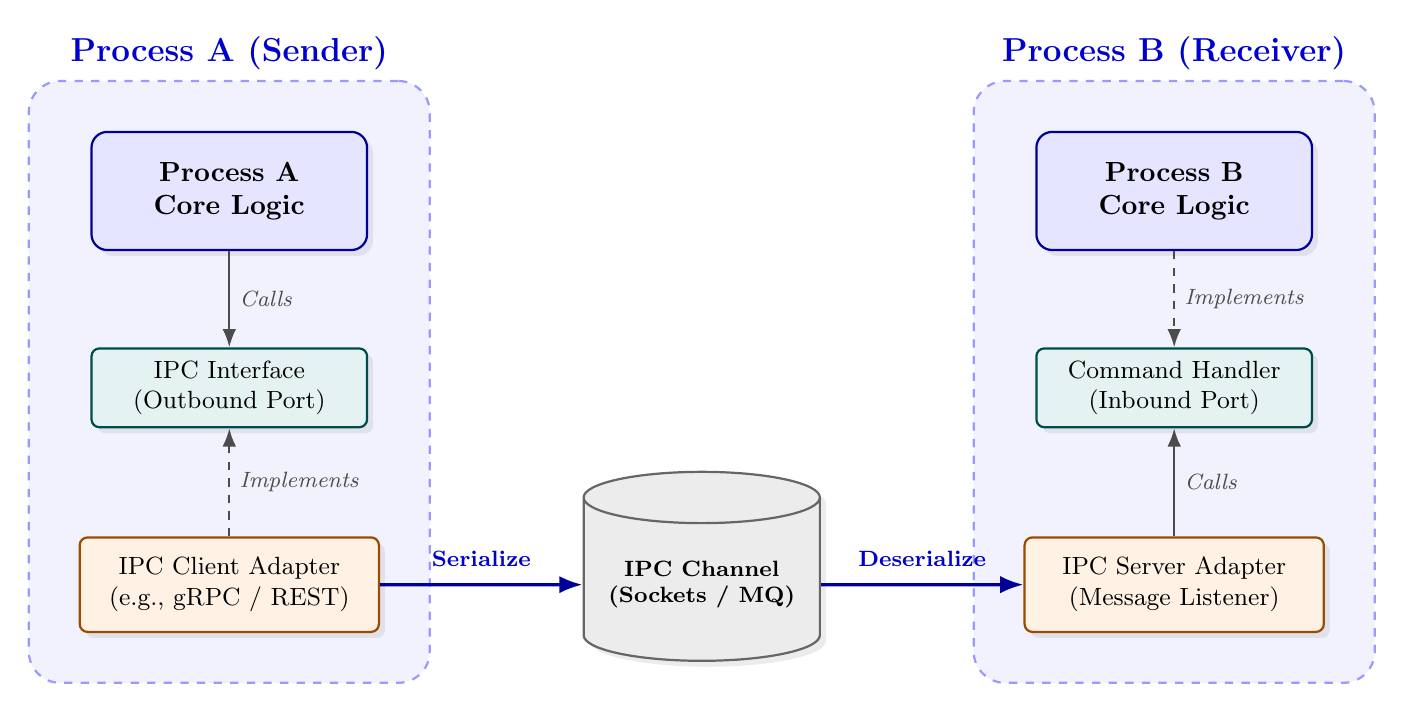
\begin{tikzpicture}[
  node distance=1.8cm,
  font=\sffamily, 
  core/.style={rectangle, rounded corners=2mm, draw=blue!60!black, thick, fill=blue!10, minimum width=3.5cm, minimum height=1.5cm, align=center, font=\bfseries, drop shadow={opacity=0.15}},
  port/.style={rectangle, rounded corners=1mm, draw=teal!60!black, thick, fill=teal!10, minimum width=3.5cm, minimum height=1cm, align=center, font=\small, drop shadow={opacity=0.15}},
  adapter/.style={rectangle, rounded corners=1mm, draw=orange!60!black, thick, fill=orange!10, minimum width=3.8cm, minimum height=1.2cm, align=center, font=\small, drop shadow={opacity=0.15}},
  ipc/.style={cylinder, draw=gray!80!black, thick, fill=gray!15, aspect=0.25, minimum height=2.4cm, minimum width=3cm, align=center, shape border rotate=90, font=\footnotesize\bfseries, drop shadow={opacity=0.15}},
  arr/.style={->, -Latex, thick, draw=black!70},
  impl/.style={->, -Latex, dashed, thick, draw=black!70},
  labeltext/.style={font=\footnotesize\itshape, text=black!70}
]

\node[core] (coreA) at (0, 0) {Process A\\Core Logic};
\node[port] (portA) at (0, -2.5) {IPC Interface\\(Outbound Port)};
\node[adapter] (adapterA) at (0, -5) {IPC Client Adapter\\(e.g., gRPC / REST)};

\draw[arr] (coreA) -- node[right, labeltext] {Calls} (portA);
\draw[impl] (adapterA) -- node[right, labeltext] {Implements} (portA);

\node[ipc] (channel) at (6, -5) {IPC Channel\\(Sockets / MQ)};
\draw[arr, very thick, draw=blue!60!black] (adapterA) -- node[above, font=\footnotesize\bfseries, inner sep=6pt, text=blue!80!black] {Serialize} (channel);

\node[adapter] (adapterB) at (12, -5) {IPC Server Adapter\\(Message Listener)};
\node[port] (portB) at (12, -2.5) {Command Handler\\(Inbound Port)};
\node[core] (coreB) at (12, 0) {Process B\\Core Logic};

\draw[arr, very thick, draw=blue!60!black] (channel) -- node[above, font=\footnotesize\bfseries, inner sep=6pt, text=blue!80!black] {Deserialize} (adapterB);
\draw[arr] (adapterB) -- node[right, labeltext] {Calls} (portB);
\draw[impl] (coreB) -- node[right, labeltext] {Implements} (portB);

\begin{pgfonlayer}{background}
  \node[draw=blue!40, thick, dashed, rounded corners=4mm, fill=blue!5, fit=(coreA) (portA) (adapterA), inner sep=18pt, label={[font=\bfseries\large, text=blue!80!black]above:Process A (Sender)}] {};
  
  \node[draw=blue!40, thick, dashed, rounded corners=4mm, fill=blue!5, fit=(coreB) (portB) (adapterB), inner sep=18pt, label={[font=\bfseries\large, text=blue!80!black]above:Process B (Receiver)}] {};
\end{pgfonlayer}

\end{tikzpicture}
}
\caption{Inter-Process Communication flow. Core business logic is strictly isolated from network and serialization layers via Interface Ports.}
\end{figure}

\end{document}
